\chapter{Browser Extension and User Testing}
\label{chap:browser-extension}

\section{Introduction}

This chapter describes how the selected HYB-MS+10\% model was used in a
working browser extension and how the browser-specific decisions were tested.
The classifier score, the extension policy, and user feedback are reported as
separate forms of evidence. This separation is important because a browser can
change how a score is presented without changing the underlying model.

\section{Local Detection Process}

The extension is implemented for Chromium-based browsers using Manifest~V3.
The three frozen hybrid checkpoints were converted to ONNX and packaged with
the same character vocabulary, maximum length, lexical-feature definitions,
and scaling values used in Python. For each HTTP(S) navigation, the extension
normalises the URL, forms the character and 35-feature inputs, obtains the
three scores, and uses their mean as the ensemble score. Inference is performed
on the user's device.

The browser policy then converts the score into an action. Secondary-review
and caution results use non-blocking notices. High-risk and very-high-risk
results pause navigation in Normal mode, whereas Warnings-only mode never
pauses the page. A user can continue once or permanently allow an exact
hostname; neither action changes the raw model score. Redirect destinations
and single-page application history changes are evaluated as new destinations.

\begin{table}[htbp]
\centering
\caption{Browser decision tiers and their user-facing behaviour.}
\label{tab:browser-tiers}
\small
\begin{tabular}{@{}p{0.20\textwidth}p{0.24\textwidth}p{0.45\textwidth}@{}}
\toprule
Tier & Normal-mode action & Purpose \\
\midrule
Allow & No notice & No strong URL-text warning was found. \\
Secondary review & Passive notice & An unusual URL can be reviewed without interruption. \\
Caution & Passive notice & Suspicious evidence is shown while the page remains available. \\
Warning & Navigation pause & A high-risk result is blocked, with a clear user override. \\
Block & Navigation pause & A very-high-risk result is blocked; the user may return, continue once, or allow the exact hostname. \\
\bottomrule
\end{tabular}
\end{table}

\section{Explainability and User Control}

The extension provides short diagnostic reasons derived from the same lexical
inputs used by the hybrid model, such as unusual length, many symbols, deep
paths, encoded characters, explicit ports, IP-address hosts, and suspicious
terms. These messages are debugging clues rather than causal explanations or
proof of phishing. They are displayed inside the extension popup and on the
full warning page. The smaller notice placed over an ordinary webpage shows
only the result, exact hostname, and risk score, with a prompt to open the
extension for details. This reduces interruption and keeps the detailed reason
available when the user requests it.

The permanent allow action now names the exact hostname, for example
``Always allow \nolinkurl{docs.google.com}'', rather than using an ambiguous
phrase such as ``allow this site''. Hostnames remain left-to-right in both the
English and Arabic interfaces. Allowing a hostname suppresses later browser
interventions for that exact name only; it does not include look-alike names or
other subdomains.

\subsection{Interface examples}

Figure~\ref{fig:browser-popup-ip} shows the compact interface used during
ordinary browsing. The first view presents a legitimate university page with
no warning. The second demonstrates the separate local-IP rule: the raw model
score remains visible, but a valid private-network address is not blocked from
URL text alone.

\begin{figure}[htbp]
\centering
\begin{minipage}[t]{0.42\textwidth}
    \centering
    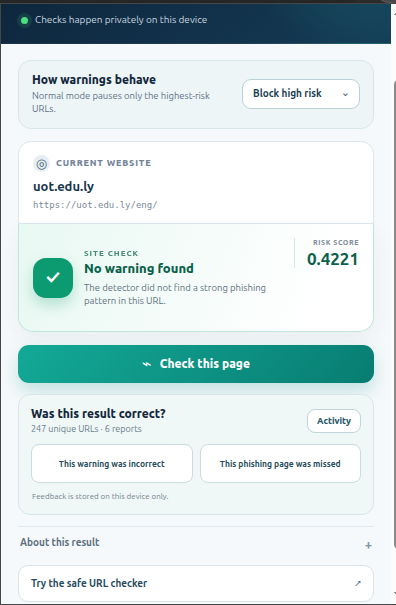
\includegraphics[width=\linewidth]{screenshots/extension_popup.png}\\[2mm]
    \small (a) Ordinary extension result
\end{minipage}
\hfill
\begin{minipage}[t]{0.42\textwidth}
    \centering
    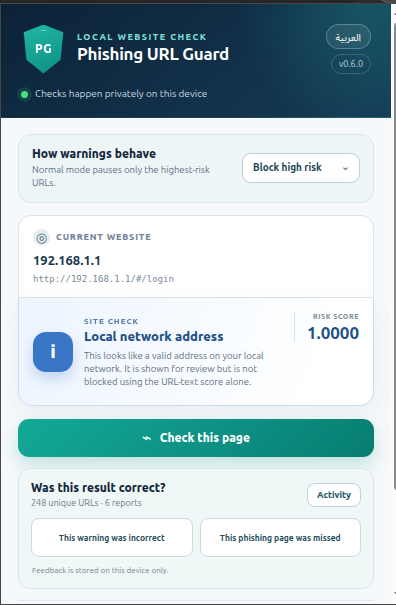
\includegraphics[width=\linewidth]{screenshots/ip_address.png}\\[2mm]
    \small (b) Private-network address handling
\end{minipage}
\caption{Extension popup examples for a normal website and a local IP address.}
\label{fig:browser-popup-ip}
\end{figure}

Figure~\ref{fig:browser-normal-warning} shows the full interruption page used
for a very-high-risk result in Normal mode. It displays the destination and
risk tier and offers three explicit choices: return to safety, continue once,
or allow only the exact hostname.

\begin{figure}[htbp]
    \centering
    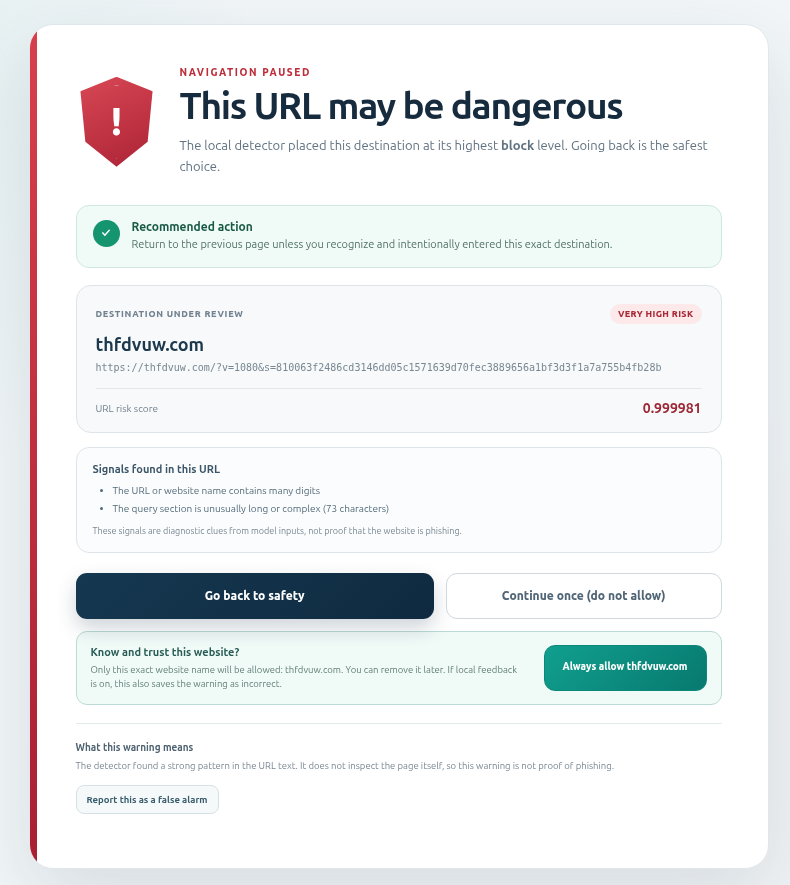
\includegraphics[width=0.82\textwidth]{screenshots/normal_mode_warning.png}
    \caption{Full warning page shown when Normal mode pauses a very-high-risk URL.}
    \label{fig:browser-normal-warning}
\end{figure}

Figure~\ref{fig:browser-passive-warning} illustrates the same type of model
result in Warnings-only mode. The destination remains available and a compact
notice is displayed instead of redirecting the tab.

\begin{figure}[htbp]
    \centering
    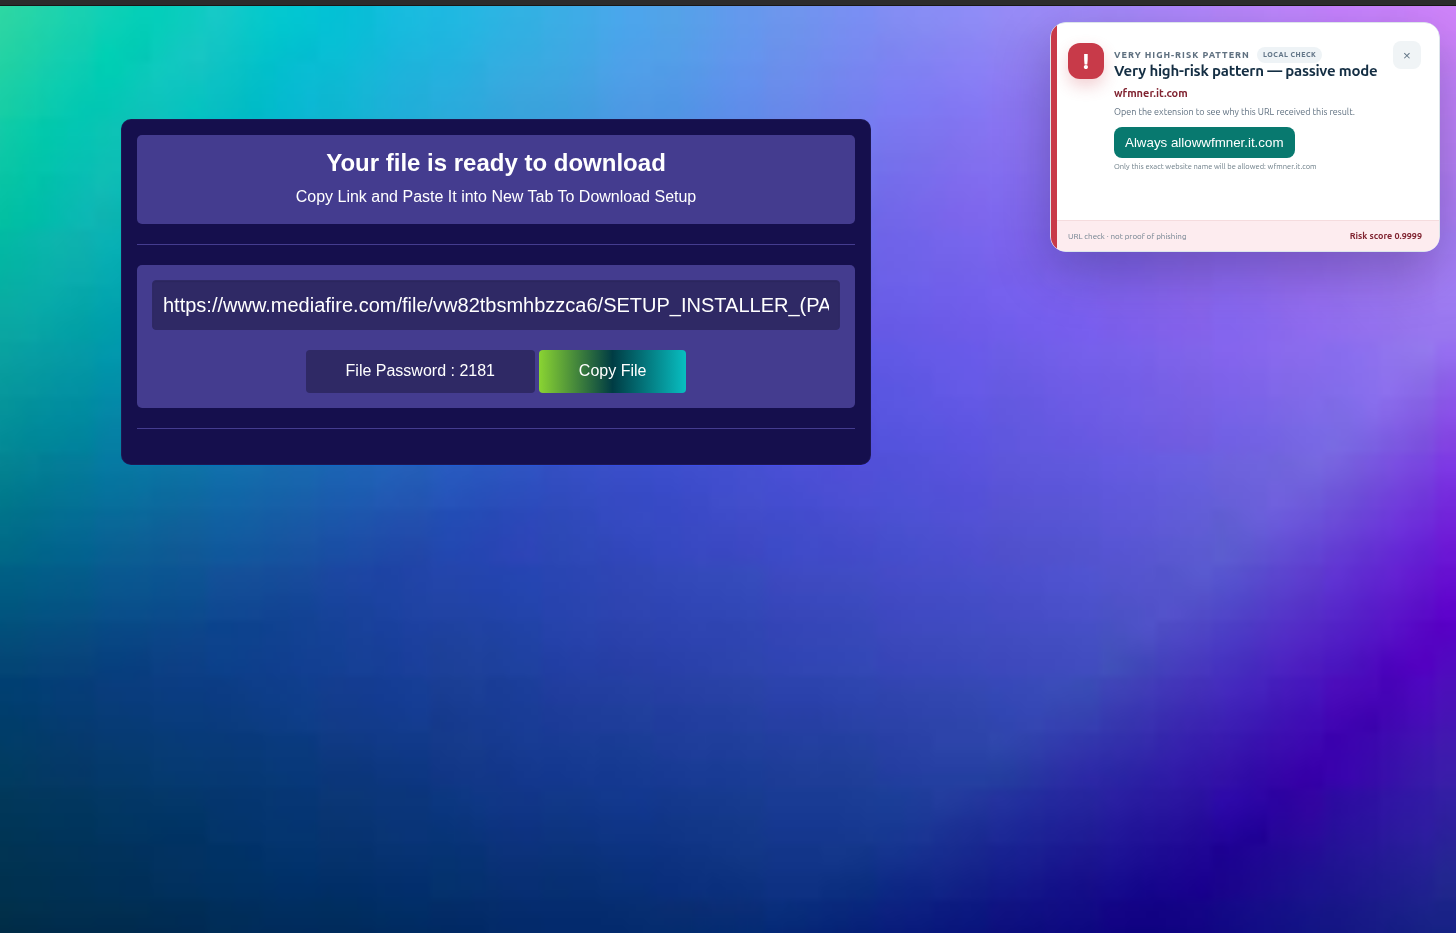
\includegraphics[width=\textwidth]{screenshots/passive_mode.png}
\caption{Non-blocking notice for a very-high-risk result in Warnings-only mode.}
\label{fig:browser-passive-warning}
\end{figure}

\clearpage

\section{Reviewed Services and User-Controlled Content}

A versioned catalogue reduces repeated false warnings on reviewed first-party
service pages. Popularity alone does not grant trust. A rule requires HTTPS,
an exact hostname, a standard port, no embedded credentials, and an allowed
path. Outbound redirect routes and other excluded paths retain normal model
handling.

ChatGPT is included through exact rules for \nolinkurl{chatgpt.com},
\nolinkurl{www.chatgpt.com}, and the legacy
\nolinkurl{chat.openai.com} hostname. The home page, conversation routes under
\texttt{/c/}, authentication, settings, login, and sign-up routes are treated
as fixed service pages. Public \texttt{/share/} pages and custom
\texttt{/g/} routes remain model-checked because their content can be created
or configured by users. Automated policy tests confirmed that normal ChatGPT
conversation URLs are allowed quietly under the current catalogue.

\section{Reliability and Privacy Controls}

Browser navigation can generate repeated events for the same URL. The
extension serialises overlapping checks, reuses a recent result for the same
tab and URL, and keeps a salted local fingerprint so a repeated assessment is
not counted as a new unique URL. Model executions, unique URL decisions,
advisory displays, and actual navigation interruptions are stored as separate
counters.

User-evaluation recording is optional and begins only after consent. Ordinary
visited URLs are not exported as readable text. A readable URL is retained
only after an explicit false-alarm or missed-phishing report, and its query
values and fragment are removed. Nothing is uploaded automatically; users
export their local results voluntarily.

\section{User Evaluation}

\subsection{Method and browsing context}

The user evaluation was designed to test the extension during ordinary
browsing and to identify usability problems that are difficult to reproduce
with a fixed dataset. Ten current-format exports were collected from Chrome,
Chromium, Opera GX, Brave, and Edge. Four participants also deliberately
visited phishing or security-testing material. Two stated that they had not
intentionally visited phishing pages, while the remaining browsing context was
not separately confirmed. This context matters because an alert produced
during deliberate phishing testing cannot automatically be called a false
alarm.

The extension records a unique canonical URL assessment rather than every
model execution. Repeated checks of the same canonical URL therefore do not
increase the unique-URL counter. A unique URL is not the same as a unique
website: different paths under one hostname can be counted separately. This
distinction is especially important for the Edge participant, who mainly used
five or six websites but generated 2,524 distinct URL paths.

Table~\ref{tab:browser-user-participants} retains the participant-level
results. ``Explicit FP'' means that the participant used the false-alarm
feedback action. ``Confirmed FP'' is used only for the Brave participant, who
stated that no phishing page was visited and confirmed all 36 alerts as false,
although the individual URLs were not stored. The four participants marked
with an asterisk deliberately tested phishing or security URLs.

\begin{table}[htbp]
\centering
\caption{Participant-level browser user-evaluation results.}
\label{tab:browser-user-participants}
\scriptsize
\resizebox{\textwidth}{!}{%
\begin{tabular}{@{}llrrrrr@{}}
\toprule
Participant & Context & Unique URLs & Alerts & Explicit FP & Confirmed FP & Reported FN \\
\midrule
Brave(S) & No intentional phishing & 218 & 36 & 0 & 36 & 0 \\
Chrome(A)$^{*}$ & Phishing/security testing & 221 & 45 & 19 & 0 & 0 \\
Chrome(AL) & Context unconfirmed & 250 & 45 & 15 & 0 & 0 \\
Chrome(B) & Context unconfirmed & 702 & 55 & 10 & 0 & 0 \\
Chrome(Mo)$^{*}$ & Phishing/security testing & 201 & 46 & 18 & 0 & 3 \\
Chrome(Mo2)$^{*}$ & Phishing/security testing & 301 & 54 & 20 & 0 & 4 \\
Chrome2(M) & No intentional phishing & 202 & 21 & 10 & 0 & 0 \\
Chromium(M) & Context unconfirmed & 276 & 30 & 10 & 0 & 0 \\
Edge(AL) & Context unconfirmed & 2,524 & 18 & 2 & 0 & 0 \\
GX(A)$^{*}$ & Phishing/security testing & 407 & 68 & 34 & 0 & 0 \\
\midrule
Total & & 5,302 & 418 & 138 & 36 & 7 \\
\bottomrule
\end{tabular}}
\par\vspace{1.5mm}
\begin{minipage}{\textwidth}
\footnotesize\textit{Note:} An asterisk ($^{*}$) identifies a participant who
intentionally tested phishing or security-related URLs.
\end{minipage}
\end{table}

\subsection{Recorded outcomes}

The current-format exports contained 5,302 unique URL observations and 418
caution, warning, or block decisions. Users submitted 138 explicit
false-alarm reports and seven missed-phishing reports. The explicit
user-reported false-alarm rate was therefore $138/5302=2.60\%$, while the
overall alert rate was $418/5302=7.88\%$. Including the 36 aggregate false
alerts confirmed by the Brave participant gives a descriptive lower-bound
false-alarm burden of $174/5302=3.28\%$.

\begin{table}[htbp]
\centering
\caption{Summary of current-format browser user-evaluation observations.}
\label{tab:browser-user-evaluation}
\begin{tabular}{@{}lr@{}}
\toprule
Recorded quantity & Count or rate \\
\midrule
User exports with a current-schema URL denominator & 10 \\
Unique URL observations & 5,302 \\
Caution, warning, or block decisions & 418 \\
Explicit false-alarm reports & 138 \\
Explicit missed-phishing reports & 7 \\
Explicit user-reported false-alarm rate & 2.60\% \\
Overall alert rate & 7.88\% \\
False-alarm lower bound including confirmed aggregate events & 3.28\% \\
\bottomrule
\end{tabular}
\end{table}

Two earlier version~0.5.0 exports were preserved rather than discarded. They
contained 41 alerts, six explicit false-alarm reports, and no reported missed
threats. Their schema did not provide a compatible unique-URL denominator, so
they are excluded from the rates above. Across current and legacy exports,
explicit reports contained 144 false alarms and seven missed threats. Adding
the 36 confirmed aggregate Brave events gives 180 observed false-alarm events,
but it does not make the unreported alerts correct by assumption.

These values are not classifier accuracy, precision, recall, FPR, or FNR.
Labels were supplied only when a user reported an outcome, and they were not
independently adjudicated in every case. The observations are therefore used
to identify warning burden, repeated false-positive patterns, and interface
problems. Formal model metrics remain based on the labelled frozen datasets in
Chapter~6.

\subsection{Reported error categories}

The feedback nevertheless revealed useful error groups. Frequently reported
cases included login and account pages, technical documentation, long service
URLs, Google Workspace links, AI services, and security-learning websites.
These findings led to exact-host display in the allow action, simpler notices,
deduplicated counting, the reviewed-service catalogue, and the corrected
shared-content policy. User feedback was therefore useful for improving the
browser layer even though it could not replace labelled classifier evaluation.

\begin{table}[htbp]
\centering
\caption{Categories of retained user-reported or participant-confirmed outcomes.}
\label{tab:browser-user-categories}
\small
\begin{tabular}{@{}lrr@{}}
\toprule
Category & False alarms & Missed threats \\
\midrule
Unspecified (individual URL not stored) & 36 & 0 \\
Login, account, and webmail & 25 & 0 \\
Other websites & 24 & 0 \\
Technical documentation and research & 21 & 0 \\
Work and online services & 17 & 0 \\
Google and Workspace & 15 & 0 \\
AI services & 13 & 0 \\
Security learning and testing & 13 & 0 \\
Shopping, media, and games & 11 & 0 \\
Education, government, and jobs & 5 & 0 \\
Reported missed threat & 0 & 7 \\
\midrule
Total & 180 & 7 \\
\bottomrule
\end{tabular}
\end{table}

\begin{figure}[htbp]
\centering
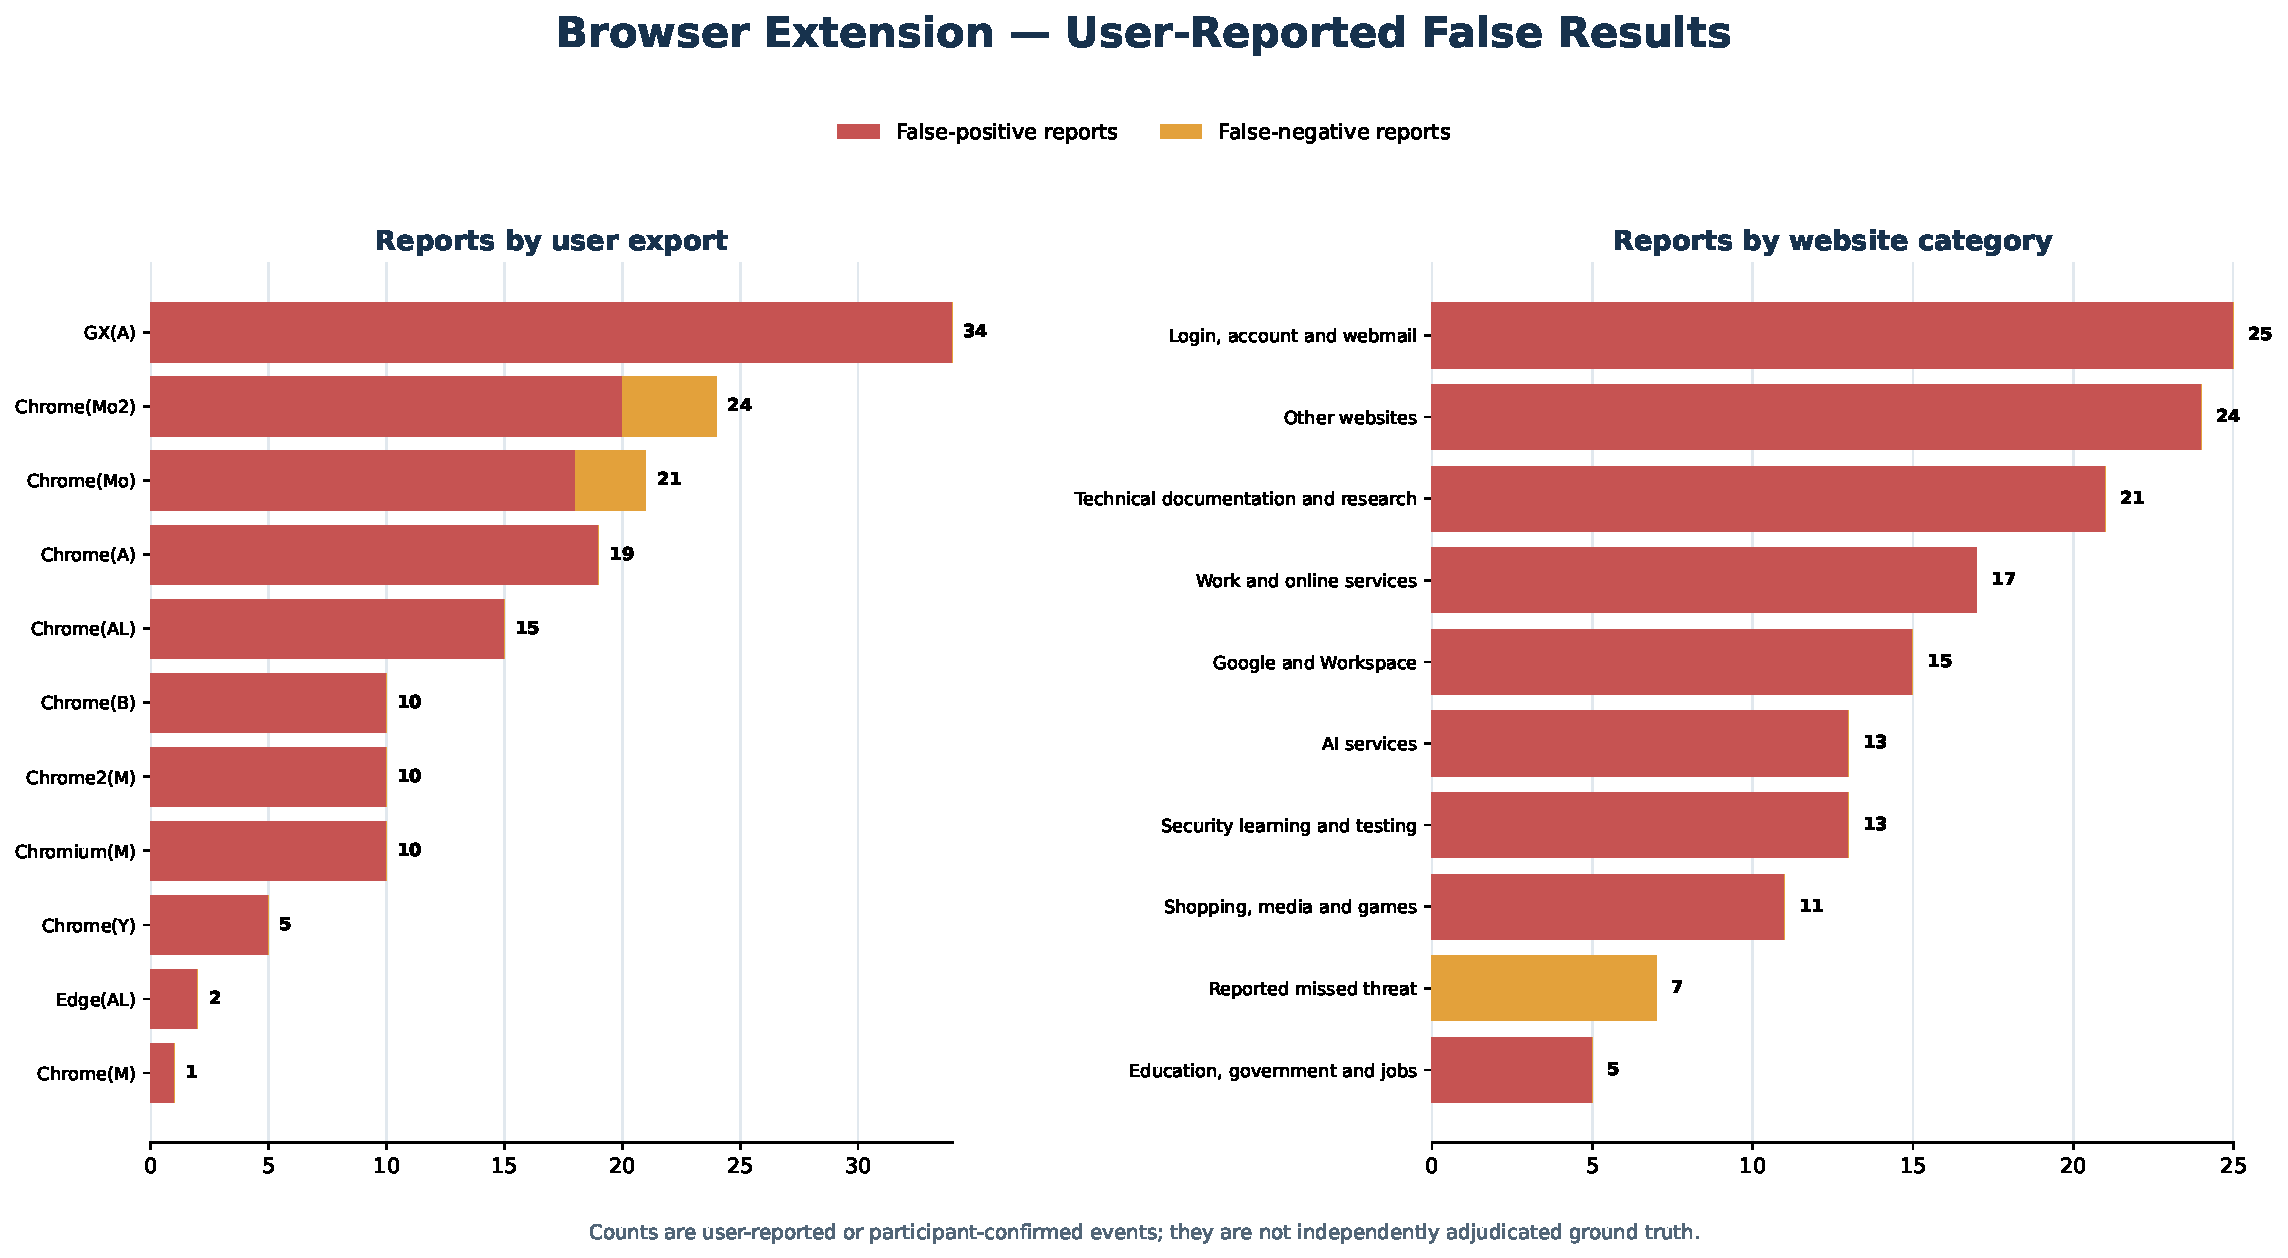
\includegraphics[width=\textwidth]{graphs/user_false_reports_by_user_and_category.pdf}
\caption{Retained user-reported and participant-confirmed outcomes by export and website category. These counts are feedback observations, not independently verified test labels.}
\label{fig:browser-user-reported-outcomes}
\end{figure}

\section{Technical Verification}

The extension build passed preprocessing parity tests, ONNX numerical parity
tests, policy and localisation tests, privacy and deduplication tests,
JavaScript syntax checks, a headless Chrome smoke test, and browser-navigation
tests using locally fulfilled pages. ONNX score disagreement with the Python
implementation was below $2.4\times10^{-7}$ in the registered parity test. The
current policy test confirms fixed-service handling, non-blocking caution
notices, blocking of high-risk tiers in Normal mode, English and Arabic
operation, and exact-host allow behaviour.

Passing these tests establishes implementation consistency, not permanent
deployment readiness. The extension remains a graduation-project prototype
whose URL-only model can produce false warnings and miss phishing under later
distributions. Reputation, page content, certificates, and live infrastructure
are outside the deployed classifier's evidence.

\section{Chapter Summary}

The browser extension runs the selected three-seed hybrid ensemble locally and
turns its score into tiered, user-controllable actions. Reliability controls
prevent repeated browser events from inflating the recorded number of unique
URLs, while consent and local storage limit collection of browsing data.

Normal ChatGPT conversation routes are recognised service pages, while public
shares and custom GPT routes remain checked. User feedback identified
recurring false-warning categories and guided usability improvements, but
labelled frozen sets remain the basis for formal performance claims.
